 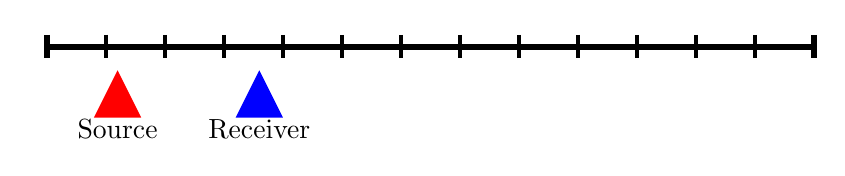
\begin{tikzpicture}[scale=1.5]
      \draw[color=black,line width=2.1](0.0,0.0) -- (6.5,0);
      %\draw[color=blue, line width=10] (0,-0.02) node {$\bullet$} ;
      %\draw[color=blue, line width=10] (5,-0.02) node {$\bullet$} ;
     % \draw node[color=blue,fill,circle,minimum size=0.01](1,1) {};
      \node[anchor=south east, color=black]
      at (0,0) {};
      %\node[anchor=south west, color=black]
      %at (4.0,0.2) {\Large $\velocity$ ?};

      \pgfmathsetmacro{\x}{0.0}
      \draw[color=black,line width=2.1](\x,0.1) -- (\x,-0.1);

      \pgfmathsetmacro{\x}{6.5}
      \draw[color=black,line width=2.1](\x,0.1) -- (\x,-0.1);

      \pgfmathsetmacro{\x}{0.5}
      \draw[color=black,line width=1.5](\x,0.1) -- (\x,-0.1);
      \draw[color=black,line width=1.5](\x,0.1) -- (\x,-0.1);



      \pgfmathsetmacro{\x}{1.0}
      \draw[color=black,line width=1.5](\x,0.1) -- (\x,-0.1);
      \pgfmathsetmacro{\x}{1.5}

      \draw[color=black,line width=1.5](\x,0.1) -- (\x,-0.1);
      \pgfmathsetmacro{\x}{2.0}
      \draw[color=black,line width=1.5](\x,0.1) -- (\x,-0.1);
      \pgfmathsetmacro{\x}{2.5}
      \draw[color=black,line width=1.5](\x,0.1) -- (\x,-0.1);
      \pgfmathsetmacro{\x}{3.0}
      \draw[color=black,line width=1.5](\x,0.1) -- (\x,-0.1);
      \pgfmathsetmacro{\x}{3.5}
      \draw[color=black,line width=1.5](\x,0.1) -- (\x,-0.1);
      \pgfmathsetmacro{\x}{4.0}
      \draw[color=black,line width=1.5](\x,0.1) -- (\x,-0.1);
      \pgfmathsetmacro{\x}{4.5}
      \draw[color=black,line width=1.5](\x,0.1) -- (\x,-0.1);
            \pgfmathsetmacro{\x}{5.0}
      \draw[color=black,line width=1.5](\x,0.1) -- (\x,-0.1);

            \pgfmathsetmacro{\x}{5.5}
      \draw[color=black,line width=1.5](\x,0.1) -- (\x,-0.1);


            \pgfmathsetmacro{\x}{6.0}
      \draw[color=black,line width=1.5](\x,0.1) -- (\x,-0.1);

      \pgfmathsetmacro{\x}{1.8}
      \pgfmathsetmacro{\dx}{0.2}
      \pgfmathsetmacro{\y}{-0.2}
      \pgfmathsetmacro{\dy}{-0.4}
      \node (A) at (\x,\y) {}; % B = 5
      \node (B) at (\x+\dx,\y+\dy) {}; % AC = 3
      \node (C) at (\x-\dx,\y+\dy) {}; % BC = 4
      \node (receiver) at (\x,\y+\dy-0.1) {Receiver}; % BC = 4
     % \draw (A) -- (B) -- (C) -- (A);
      \begin{scope}%[on background layer]
        \fill [blue] (A.center) -- (B.center) -- (C.center) -- cycle;
      \end{scope}

            \pgfmathsetmacro{\x}{0.6}
      \pgfmathsetmacro{\dx}{0.2}
      \pgfmathsetmacro{\y}{-0.2}
      \pgfmathsetmacro{\dy}{-0.4}
      \node (A) at (\x,\y) {}; % B = 5
      \node (B) at (\x+\dx,\y+\dy) {}; % AC = 3
      \node (C) at (\x-\dx,\y+\dy) {}; % BC = 4
      \node (source) at (\x,\y+\dy-0.1) {Source}; % BC = 4
      %\draw [red] (A) -- (B) -- (C) -- (A);
      \begin{scope}%[on background layer]
        \fill [red] (A.center) -- (B.center) -- (C.center) -- cycle;
      \end{scope}
\end{tikzpicture}
